\documentclass[
oneside,
openany,
bibliography=totoc,
version=first,
parskip,
12pt,
numbers=noenddot
]{scrbook}

\usepackage{scrhack}
%\usepackage{background} % Draft Watermark

% Encoding
\usepackage[T1]{fontenc}
\usepackage[utf8]{inputenc}

% Grammar
\usepackage[british]{babel}
%\usepackage[ngerman]{babel}

% Layout
\usepackage{scrpage2} 
\usepackage[section]{placeins} % Keep figures in section
\usepackage[top=2cm, left=2cm, right=2cm, bottom=2cm]{geometry} % Paper borders. If writing a thesis, change left border to 4cm
\usepackage[onehalfspacing]{setspace}

% Listings
\usepackage{listings}
\lstset{literate=
  {á}{{\'a}}1 {é}{{\'e}}1 {í}{{\'i}}1 {ó}{{\'o}}1 {ú}{{\'u}}1
  {Á}{{\'A}}1 {É}{{\'E}}1 {Í}{{\'I}}1 {Ó}{{\'O}}1 {Ú}{{\'U}}1
  {à}{{\`a}}1 {è}{{\`e}}1 {ì}{{\`i}}1 {ò}{{\`o}}1 {ù}{{\`u}}1
  {À}{{\`A}}1 {È}{{\'E}}1 {Ì}{{\`I}}1 {Ò}{{\`O}}1 {Ù}{{\`U}}1
  {ä}{{\"a}}1 {ë}{{\"e}}1 {ï}{{\"i}}1 {ö}{{\"o}}1 {ü}{{\"u}}1
  {Ä}{{\"A}}1 {Ë}{{\"E}}1 {Ï}{{\"I}}1 {Ö}{{\"O}}1 {Ü}{{\"U}}1
  {â}{{\^a}}1 {ê}{{\^e}}1 {î}{{\^i}}1 {ô}{{\^o}}1 {û}{{\^u}}1
  {Â}{{\^A}}1 {Ê}{{\^E}}1 {Î}{{\^I}}1 {Ô}{{\^O}}1 {Û}{{\^U}}1
  {œ}{{\oe}}1 {Œ}{{\OE}}1 {æ}{{\ae}}1 {Æ}{{\AE}}1 {ß}{{\ss}}1
  {ű}{{\H{u}}}1 {Ű}{{\H{U}}}1 {ő}{{\H{o}}}1 {Ő}{{\H{O}}}1
  {ç}{{\c c}}1 {Ç}{{\c C}}1 {ø}{{\o}}1 {å}{{\r a}}1 {Å}{{\r A}}1
  {€}{{\EUR}}1 {£}{{\pounds}}1
}

\lstset{ %
  backgroundcolor=\color{white},   % choose the background color; you must add \usepackage{color} or \usepackage{xcolor}
  basicstyle=\ttfamily\lst@ifdisplaystyle\footnotesize\fi,        % the size of the fonts that are used for the code
  breakatwhitespace=false,         % sets if automatic breaks should only happen at whitespace
  breaklines=true,                 % sets automatic line breaking
  captionpos=t,                    % sets the caption-position to bottom
  commentstyle=\color{green},    % comment style
  extendedchars=true,              % lets you use non-ASCII characters; for 8-bits encodings only, does not work with UTF-8
  frame=tb,                    % adds a frame around the code
  keepspaces=true,                 % keeps spaces in text, useful for keeping indentation of code (possibly needs columns=flexible)
  keywordstyle=\color{blue},       % keyword style
  language=C,                 % the language of the code
  numbers=left,                    % where to put the line-numbers; possible values are (none, left, right)
  numbersep=5pt,                   % how far the line-numbers are from the code
  numberstyle=\tiny\color{gray}, % the style that is used for the line-numbers
  rulecolor=\color{black},         % if not set, the frame-color may be changed on line-breaks within not-black text (e.g. comments (green here))
  showspaces=false,                % show spaces everywhere adding particular underscores; it overrides 'showstringspaces'
  showstringspaces=false,          % underline spaces within strings only
  showtabs=false,                  % show tabs within strings adding particular underscores
  stepnumber=1,                    % the step between two line-numbers. If it's 1, each line will be numbered
  stringstyle=\color{purple},     % string literal style
  tabsize=2,                       % sets default tabsize to 2 spaces
  title=\lstname,                   % show the filename of files included with \lstinputlisting; also try caption instead of title
  xleftmargin=1em % otherwise the line numbers do not fit the margin
}

% Bibliography
\usepackage[
style=authoryear, % Harvard Style
backend=biber,
dashed=false
]{biblatex} 

\addbibresource{bibliography.bib} % Bibliography File

% Typography
\usepackage{amsmath}
\usepackage{amsfonts}
\usepackage{amssymb}
\usepackage[final,babel]{microtype}

% Abbreviations
\usepackage[printonlyused]{acronym}

% Numbering
\usepackage{chngcntr} % continue footnode count on new chapter
\counterwithout{footnote}{chapter} % continue footnode count on new chapter
%\setcounter{secnumdepth}{4} % subsubsection numbering
%\setcounter{tocdepth}{4}	 % add subsubsection to table of content

% Center page number at the top of the page
\deftripstyle{pgnumtopcenter}{}{\pagemark{}}{}{}{}{}
\pagestyle{pgnumtopcenter}
\renewcommand{\chapterpagestyle}{pgnumtopcenter}

% Various
\usepackage{xcolor}
\usepackage{subfigure}
\usepackage{wrapfig}
\usepackage{graphicx}
\usepackage{hyperref}
\usepackage[noabbrev]{cleveref}
\usepackage[autostyle=true,autopunct]{csquotes}
\usepackage[super]{nth} % \nth{1} = 1st nice formatted
\usepackage{lipsum}
\renewcommand{\familydefault}{\sfdefault} % Sans Serif Font

% No page break after chapter:
%\usepackage{etoolbox}
%\makeatletter
%\patchcmd{\chapter}{\if@openright\cleardoublepage\else\clearpage\fi}{}{}{}
%\makeatother

\begin{document}
\frontmatter % Roman page numbering

\begin{titlepage}
	\begin{center}
	Hochschule Rhein-Waal\\
	Fakutltät Kommunikation und Umwelt\\
	Prof. Dr. Charles Xavier\\
	\vspace{2cm}
	Essay\\
	WS 2015/16\\
	Module: Scientific Writing\\
	\vspace{3cm}
	\uppercase{\textbf{\Large{My Topic}}}\\
	\vspace{8cm}
	My Name (Matriculation Number)\\
	\vspace{1cm}
	Submission Date:\\
	21.01.2016
	\end{center}
\end{titlepage}
\newpage

\addchap*{Abstract}
\lipsum[5]
\textbf{Keywords:}\\
Keyword 1-5
\newpage

\tableofcontents
\newpage

\addchap*{Abbreviations}
\begin{acronym}[rpnx]
	% uppercase letter:
	\acro{URL}{Uniform Resource Locator} 
	% lowercase letter:
\end{acronym}

\lstlistoflistings
\clearpage
\listoftables 
\clearpage
\listoffigures
\clearpage

\mainmatter % Arabic page numbering
\acresetall % if acronyms have been used in the abstract, repeat them.

\chapter{Introduction}
\label{sec:introduction}
\lipsum[1]

\chapter{Main Part}
\label{sec:main}
\lipsum[2] and \ac{URL}

\section{Section A}
\label{sec:a}
\lipsum[3] \autocite{doe2005}

\begin{figure}[ht]
	\centering
    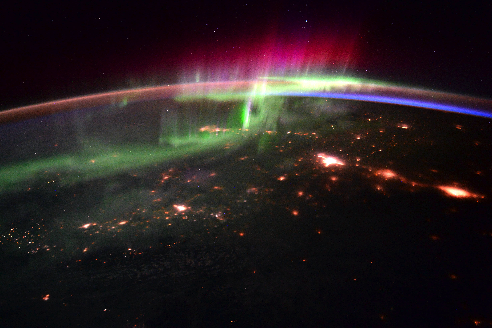
\includegraphics[width=1\textwidth]{figures/aurora.jpg}
	\caption{Aurora and the Pacific Northwest \emph{Image Credits: ESA/NASA}}
	\label{fig:aurora}
\end{figure}

\url{http://www.nasa.gov/image-feature/aurora-and-the-pacific-northwest}

\section{Section B}
\label{sec:b}
\lipsum[4] \textcite{doe2005}

\begin{singlespace}
\begin{lstlisting}[caption=C Hello World, label=lst:hello_world]
#include <stdio.h>

int main(void)
{
	printf("Hello, World\n");
    return 0;
}
\end{lstlisting}
\end{singlespace}

\chapter{Conclusion}
\label{sec:conclusion}
\lipsum[1]

\printbibliography
\appendix
\chapter{Appendix 1}

\newpage
\chapter*{Declaration of Authority}
English\\
I, <name>, hereby declare that the work presented herein is my own work
completed without the use of any aids other than those listed. Any material
from other sources or works done by others has been given due
acknowledgement and listed in the reference section. Sentences or parts of
sentences quoted literally are marked as quotations; identification of other
references with regard to the statement and scope of the work is quoted.
The work presented herein has not been published or submitted elsewhere
for assessment in the same or a similar form. I will retain a copy of this
assignment until after the Board of Examiners has published the results,
which I will make available on request.

German\\
Hiermit erkläre ich, <Name>, dass ich die hier vorliegende Arbeit selbstständig
und ohne unerlaubte Hilfsmittel angefertigt habe. Informationen, die
anderen Werken oder Quellen dem Wortlaut oder dem Sinn nach entnommen
sind, habe ich kenntlich gemacht und mit exakter Quellenangabe
versehen. Sätze oder Satzteile, die wörtlich übernommen wurden, wurden
als Zitate gekennzeichnet. Die hier vorliegende Arbeit wurde noch an
keiner anderen Stelle zur Prüfung vorgelegt und weder ganz noch in
Auszügen veröffentlicht. Bis zur Veröffentlichung der Ergebnisse durch den
Prüfungsausschuss werde ich eine Kopie dieser Studienarbeit aufbewahren
und wenn nötig zugänglich machen.

<Ort, Datum> <Unterschrift>

\backmatter
\end{document}
